\chapter{Another Chapter}

This is another chapter and it has a table. You can reference Table \ref{tab:a_table} using the command \ref{tab:a_table}.

\section{Tables}

\begin{table}[ht]
    \centering
    \begin{tabular}{cc}
         \textbf{X} & \textbf{Y}  \\ \toprule
         1 & 2 \\
         1 & 2 \\
         1 & 2 \\ \bottomrule
    \end{tabular}
    \caption{This is a table.}
    \label{tab:a_table}
\end{table}


\section{Figures}

This chapter also has a figure (see Figure \ref{fig:a_figure}).

\begin{figure}[ht]
    \centering
    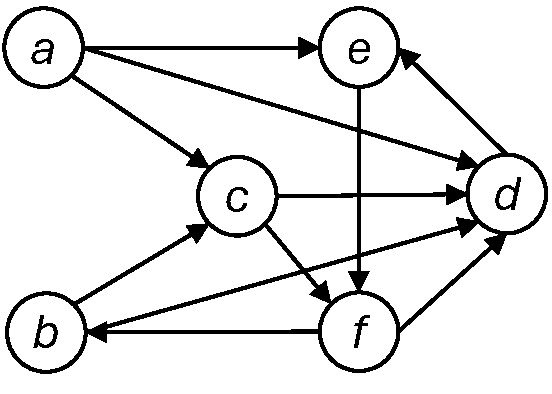
\includegraphics[width=0.5\linewidth]{figures/g1.pdf}
    \caption{A figure showing a directed graph. Prefer vectorized formats like PDF and EPS instead of JPG and PNG.}
    \label{fig:a_figure}
\end{figure}